\documentclass{standalone}
\usepackage{tikz}
\usetikzlibrary{arrows.meta, positioning}

\begin{document}
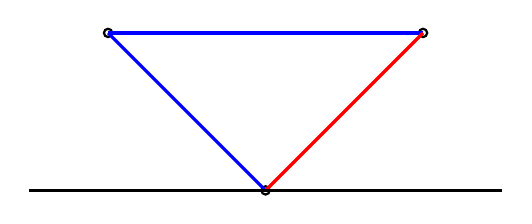
\begin{tikzpicture}[scale=2]
  % Node Styles
  \tikzset{
    node/.style={circle, draw, thick, minimum size=3pt, inner sep=0, fill=white}
  }
  
  % Define Coordinates for Nodes
  \coordinate (A) at (-1, 1);
  \coordinate (B) at (1, 1);
  \coordinate (C) at (0, 0);
  
  % Draw Nodes
  \foreach \point in {A,B,C} {
    \node[node] at (\point) {};
  }
  
  % Draw Edges
  \draw[blue, very thick] (A) -- (B);
  \draw[blue, very thick] (A) -- (C);
  \draw[red, very thick] (B) -- (C);
  \draw[black, very thick] (-1.5, 0) -- (1.5, 0);
\end{tikzpicture}
\end{document}